% !Mode:: "TeX:UTF-8"
% !TEX program = xelatex
\documentclass[cs4size,a4paper,fancyhdr,fntef,oneside,openany]{ctexbook}
\usepackage[a4paper,top=51pt,bottom=51pt,left=68pt,right=57pt,headsep=14pt,footskip=26pt,includehead, includefoot]{geometry}
\title{你好,\LaTeX}
\author{Monster,Bruce}
\makeatletter
\let\OLDappendix\appendix
\newif\if@appendixinbackmatter
\renewenvironment{appendix}
{
  \if@mainmatter
     \@appendixinbackmatterfalse\OLDappendix
  \else
      \@appendixinbackmattertrue\@mainmattertrue\OLDappendix
 \fi
}
\makeatother
\begin{document}
\maketitle
\frontmatter
\tableofcontents
\mainmatter
% !TEX root = ../main.tex

\chapter{绪论\texorpdfstring{\footnote{章标题中脚注命令测试}}{}(or 引言)各种测试}
绪论占坑,但是也要测试到底占多少缩进,换行情况,行距,都是这些不听话的小伙伴,好好调教你们。

\section{列表环境\texorpdfstring{\footnote{节标题中脚注命令测试}}{}测试}
以下是一个测试用的列表环境,内容不要在意。\footnote{正文中中脚注命令测试,长脚注情况:这包括如下事实:“未经本人同意,监听、录制或转播私人性质的谈话或秘密谈话;未经本人同意,拍摄、录制或转播个人在私人场所的形象”}

这里测试列表标签功能的交叉引用格式\ref{itm:11},\ref{itm:12},\ref{itm:13},\ref{itm:14},分别表示第一至第四层级的itemize系列的交叉引用情况。
\begin{enumerate}
	\item 第一级列表\label{itm:11}
	\item 第一级列表
	\begin{enumerate}
		\item 第二级列表\label{itm:12}
		\item 第二级列表
		\begin{enumerate}
			\item 第三级列表\label{itm:13}
			\item 第三级列表
			\begin{enumerate}
				\item 第四级列表\label{itm:14}
				\item 第四级列表
				\item 第四级列表
				\item 第四级列表
			\end{enumerate}
			\item 第三级列表
			\item 第三级列表
			\item 第三级列表
		\end{enumerate}
		\item 第二级列表
		\item 第二级列表
	\end{enumerate}
	\item 第一级列表
	\item 第一级列表
	\item 第一级列表
\end{enumerate}

正是由于油膜物质的发现,使“雾伞”计划成为可能,这个计划是用核爆炸在太空中蒸发和扩散油膜物质,在太阳与地球之间形成一团“油膜尘埃”,降低太阳 对地球的辐射,达到缓解地球温室效应的目的。“我记得,海王星轨道附近应该还有前战争时期的恒星型核弹吧?”肯又问。“有的,‘雾伞’工程的飞船也装载了一些,在海王星环和卫星上爆破用,具体数目不清楚。” “好像一颗就够了。”肯兴奋起来。两个世纪前面壁者雷迪亚兹的战略计划中所研制的恒星型氢弹,后来共制造了五千多颗。虽然这种武器在末日之战中作用有限,但正如雷迪亚兹所言,各大 国主要是为可能爆发的人类之间的行星际战争准备的,核弹主要在大低谷时期制造,那时由于资源的匮乏,国际关系极其紧张,人类自身的战争一触即发。进入新时期后,这些骇人听闻的武器成了危险的鸡肋,虽然其所有权都属于地球国家, 但还是都被送入太空存贮,少部分已经用于行星工程的爆破,还有一部分送入太阳系外围轨道。曾有人设想将核弹中的聚变材料可以作为远程飞船的燃料补充,但由于核弹的拆解很困难,这个设想一直没有真正实现过\footnote{看看另起一页脚注编号的变化}。
\begin{itemize}
	\item 第一级列表
	\item 第一级列表
	\begin{itemize}
		\item 第二级列表
		\item 第二级列表
		\begin{itemize}
			\item 第三级列表
			\item 第三级列表
			\begin{itemize}
				\item 第四级列表
				\item 第四级列表
				\item 第四级列表
				\item 第四级列表
			\end{itemize}
			\item 第三级列表
			\item 第三级列表
			\item 第三级列表
		\end{itemize}
		\item 第二级列表
		\item 第二级列表
	\end{itemize}
	\item 第一级列表
	\item 第一级列表
	\item 第一级列表
\end{itemize}

“你觉得能行,”罗宾逊两眼放光地问道,他后悔这么简单的事自己怎么没 想到,一个载入史册的机会让肯抢去了。“试试吧,只有这一个办法了。”“如果行,博士,以后林格一斐兹罗监测站将永远按产生1G重力的速度旋转。”“这可是人类造出来的最大的东西了。”“蓝影”号飞船的指令长看着舱外漆黑的太空说,他极力想象自己能看到尘埃云,但确实什么\footnote{连续两个脚注测试1}\footnote{连续两个脚注测试2}
\begin{enumerate}
	\item 第四级列表
	\item 第四级列表
	\begin{enumerate}
		\item 第五级列表
		\item 第五级列表
		\item 第五级列表
	\end{enumerate}
	\item 第四级列表
	\item 第四级列表
\end{enumerate}
都看不到。“为什么它不能被阳光照出来呢,就像彗星的尾巴那样...”飞船驾驶员说,“蓝影”号上只有他和指令长两个人。他知道,尘埃云的密度确实像彗星尾一样稀薄,几乎和地球上实验室中造出的真空差不多。“可能是阳光太弱吧。”指令长回头看看太阳,在这海王星轨道和柯伊伯带 之间的冷寂空间,太阳看上去只是一颗刚能看出圆盘形状的大星星。阳光倒是还可以在舱壁上照出亮影,但已经十分微弱了。“再说,彗尾也要在一定的距离外 才能看到,我们可是就在云的边缘。”

\section{参考文献测试}
测试一下引用\cite{shi_chinas_2010},引用\cite{shi2010china,hata2014soi,muhammad2011development},还有其它引用\cite{shi2010china,muhammad2011development,lamport1994latex}.

\section{浮动体测试}
\subsection{插图测试}
如\autoref{fig:first_image_tset}是对此模版的第一张插图测试。

\begin{figure}[htbp]
	\centering
	
\includegraphics[width = 0.5\linewidth]{Chapter1.png}
	\caption{第一张插图测试}\label{fig:first_image_tset}
\end{figure}

以下是一段对这些插图来历的介绍,引用自知乎专栏All about TeXnique中夏晓昊的文章\href{http://zhuanlan.zhihu.com/LaTeX/19669122}{《The TeXbook导读:从那头(多图杀猫的)狮子说起》}。

在The TeXbook中,有着一系列的以狮子为主题的插图。这些插图的作者是Duane Bibby。也是从The TeXbook开始,不少TeX书也采取了以狮子为主的插图,作者也是Duane Bibby。另外,每年的TUG(TeX Users Group)年会都会有一张以狮子为主题的logo,这只狮子已经是社区的吉祥物了。

为什么选择狮子呢?Yannis Haralambous写道(原文法语,此为转译后的英文):Not for nothing is TeX represented by a lion. Donald Knuth has told us that lions are to him the guardians of libraries in the United States because there is a statue of a lion in front of the entrance of each large library there. Guardian of libraries, guardian of the Book—is that not indeed what TeX ultimately aspires to be? 或许吧。 (顺便说一句,TeX和MetaFont都用了狮子,TeX是公狮子,MetaFont是母狮子,多么和谐的一对啊。如果你还是忽略MetaFont的存在,那你还没有认识到它的重要性。)

作为插图,首要的一点就是贴切,然后是有趣。在TeX社区里面,have fun是一个很重要的词组,也有人说Happy TeXing。我知道有不少人不喜欢TeX,但是能有什么理由呢?如果你用不到它,那么浅尝辄止即可。如果你会用到很频繁,最好慢慢修炼做到精通。如果你只是偶尔用到,那么可以搬个模版什么的,甚至也可以找人帮你(不要指望别人会用足够的空闲时间来帮你,他没有这个义务,请支付报酬,最少也得请吃个红烧肉吧)。下面的插图,是TeX TeXbook中的,我也希望这个新年的假期,能有人有空来看看这本书。即使不能把所有的东西都看懂,那么也会对TeX的设计有了一定的了解,拿到扳手就好。

\subsection{表格测试}
在这里推荐制表采用功能强大的tabu宏包以取代其它制表宏包。具体tabu宏包的使用说明参见tabu宏包的说明文档。

以下节分别用来测试各种表格环境如,tabular,tabu,longtabu等,还有对caption格式的修改和测试。以下表格样式全部采用三线表。

\subsubsection{array宏包tabular表格环境测试}
如\autoref{tab:first_table_test}是对array宏包的tabular表格环境测试。
\begin{table}[htbp]
	\centering
	\caption{这是一个用tabular环境的测试用的表格}\label{tab:first_table_test}
    \begin{tabular}{lrr}
    \toprule
    \textbf{行星}     & \textbf{赤道半径}km & \textbf{公转周期}d \\
    \midrule
    水星     & 2.439  & 87.9 \\
    金星     & 6.1    & 224.682 \\
    地球     & 6378.14 & 365.24 \\
    \bottomrule
    \end{tabular}%
\end{table}

\subsubsection{tabu宏包表格环境测试}
如\autoref{tab:tabu_test_1}是对tabu宏包的tabu表格环境测试。在这里表格命令与\autoref{tab:first_table_test}的命令相同,只是tabular环境改成了tabu环境。
\begin{table}[htbp]
	\centering
	\caption{这是一个用tabu环境的测试用的表格}\label{tab:tabu_test_1}
    \begin{tabu}{lrr}
    \toprule
    \textbf{行星}     & \textbf{赤道半径}km & \textbf{公转周期}d \\
    \midrule
    水星     & 2.439  & 87.9 \\
    金星     & 6.1    & 224.682 \\
    地球     & 6378.14 & 365.24 \\
    \bottomrule
    \end{tabu}%
\end{table}

\autoref{tab:tabu_test_2}对tabu to表格的x列模式进行测试。在表格导言区中设置为X[1]X[2]X[2],表示这三列表格的列宽比值为1:2:2,总的表格宽度由tabu to环境设置,这里设置为0.6\textbackslash linewidth。相比于tabular环境,tabu环境的列宽设置方便许多。
\begin{table}[htbp]
	\centering
	\caption{tabu环境测试表格---X列模式}\label{tab:tabu_test_2}
    \begin{tabu} to 0.6\linewidth{X[1]X[2]X[2]}
    \toprule
    \textbf{行星}     & \textbf{赤道半径}km & \textbf{公转周期}d \\
    \midrule
    水星     & 2.439  & 87.9 \\
    金星     & 6.1    & 224.682 \\
    地球     & 6378.14 & 365.24 \\
    \bottomrule
    \end{tabu}%
\end{table}

如\autoref{tab:tabu_test_3}是longtabu环境测试表格。longtabu环境不能用在table浮动体环境中。根据GB/T 7713.1-2006规定:如果某个表需要转页接排,在随后的各页上应重复表的编号。编号后跟标题(可省略)和“(续)”,置于表上方。续表应重复表头。

特别需要注意的是,longtabu是基于longtable宏包开发的,所以在zjuthesis.cls文件中已经插入了longtable宏包。longtable环境的所有功能都可以在longtabu中使用,如\textbackslash endhead,\textbackslash endfirsthead,\textbackslash endfoot,\textbackslash endlastfoot,和\textbackslash caption等。具体用法请参见longtable和tabu宏包的相应文档。
\begin{longtabu}{lccc}
\caption{材料弹性模量及泊松比}\label{tab:tabu_test_3}\\
\toprule
名  称   & 弹性模量E/Gpa & 切变模量G/Gpa & 泊松比$\mu$ \\
\midrule%
\endfirsthead
\caption{材料弹性模量及泊松比(续)}\\
\toprule
名  称   & 弹性模量E/Gpa & 切变模量G/Gpa & 泊松比$\mu$ \\
\midrule%
\endhead
\bottomrule%
\endfoot
镍铬钢、合金钢 & 206    & 79.38  & 0.3 \\
碳 钢    &  196~206 & 79     & 0.3 \\
铸 钢    &  172~202 &        & 0.3 \\
球墨铸铁   &  140~154 &  73~76 & 0.3 \\
灰铸铁、白口铸铁 &  113~157 & 44     &  0.23~0.27 \\
冷拔纯铜   & 127    & 48     &   \\
轧制磷青铜  & 113    & 41     &  0.32~0.35 \\
轧制纯铜   & 108    & 39     &  0.31~0.34 \\
轧制锰青铜  & 108    & 39     & 0.35 \\
铸铝青铜   & 103    & 41     & 0.3 \\
冷拔黄铜   &  89~97 &  34~36 &  0.32~0.42 \\
轧制锌    & 82     & 31     & 0.27 \\
硬铝合金   & 70     & 26     & 0.3 \\
轧制铝    & 68     &  25~26 &  0.32~0.36 \\
铅      & 17     & 7      & 0.42 \\
玻璃     & 55     & 22     & 0.25 \\
混凝土    &  14~39 &  439~15.7 &  0.1~0.18 \\
纵纹木材   &  9.8~12 & 0.5    &   \\
横纹木材   &  0.5~0.98 &  0.44~0.64 &   \\
橡胶     & 0.00784 &        & 0.47 \\
电木     &  1.96~2.94 &  0.69~2.06 &  0.35~0.38 \\
赛璐珞    &  1.71~1.89 &  0.69~0.98 & 0.4 \\
可锻铸铁   & 152    &        &  \\
拔制铝线   & 69     &        &  \\
大理石    & 55     &        &  \\
花岗石    & 48     &        &  \\
石灰石    & 41     &        &  \\
尼龙1010 & 1.07   &        &  \\
夹布酚醛塑料 &  4~8.8 &        &  \\
石棉酚醛塑料 & 1.3    &        &  \\
高压聚乙烯  &  0.15~0.25 &        &  \\
低压聚乙烯  &  0.49~0.78 &        &  \\
聚丙烯    &  1.32~1.42 &        &  \\
硬聚氯乙烯  &  3.14~3.92 &        &  \\
聚四氟乙烯  &  1.14~1.42 &        &  \\
\end{longtabu}%

\subsection{子图}
这里子图的排版推荐使用subcaption宏包,不再推荐使用subfig宏包,更不推荐使用subfigure宏包。值得注意的是,在zjuthesis.cls文件中已经写入了subcaption宏包,而且subcaption宏包与subfigure和subfig宏包是相互冲突的。因此,如果你还想使用subfig宏包而不想使用subcaption宏包,请自己到zjuthesis.cls文件的相关位置更改,具体的使用及修改方法参见相应的宏包说明文档。不过在这里还是不推荐直接去更改zjuthesis.cls文档,除非你对\LaTeX 的相关命令很清楚,知道自己在改什么,并且不会对其他格式产生影响。

具体的subcaption宏包使用方法我这里不仔细介绍,以下只是对subcaption进行一些简单的测试,主要是格式调整和交叉引用。

如\autoref{fig:subfig_test1}是有两张子图的模式,对子图进行交叉引用,如\autoref{subfig:1a}和\autoref{subfig:1b}。

\begin{figure}[htbp]
	\centering
	\begin{subfigure}[b]{.4\textwidth}
		\centering
		
\includegraphics[width = \textwidth]{Chapter2.png}
		\caption{书籍排版与普通排版}\label{subfig:1a}
	\end{subfigure}
	\quad
	\begin{subfigure}[b]{.4\textwidth}
		\centering
		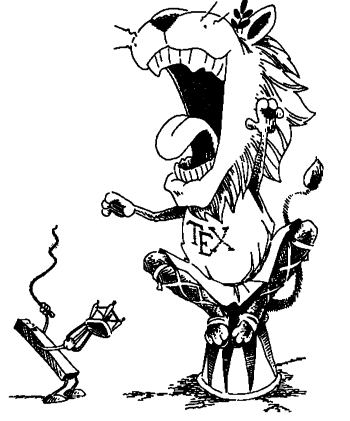
\includegraphics[width = \textwidth]{Chapter3.png}
		\caption{\TeX 的控制系列}\label{subfig:1b}
	\end{subfigure}
	\caption{子图模式测试1:2张图}\label{fig:subfig_test1}
\end{figure}

如\autoref{fig:subfig_test2}是有四张子图的模式,对子图进行交叉引用,如\autoref{subfig:2a}、\autoref{subfig:2b}、\autoref{subfig:2c}和\autoref{subfig:2d}。

\begin{figure}[htbp]
	\centering
	\begin{subfigure}[b]{.4\textwidth}
		\centering
		
\includegraphics[width = \textwidth]{Chapter4.png}
		\caption{字体}\label{subfig:2a}
	\end{subfigure}
	\begin{subfigure}[b]{.4\textwidth}
		\centering
		
\includegraphics[width = \textwidth]{Chapter5.png}
		\caption{编组}\label{subfig:2b}
	\end{subfigure}
	\begin{subfigure}[b]{.4\textwidth}
		\centering
		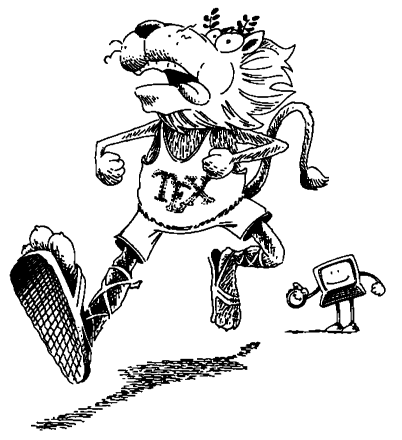
\includegraphics[width = \textwidth]{Chapter6.png}
		\caption{运行\TeX}\label{subfig:2c}
	\end{subfigure}
	\begin{subfigure}[b]{.4\textwidth}
		\centering
		
\includegraphics[width = \textwidth]{Chapter7.png}
		\caption{\TeX 工作原理}\label{subfig:2d}
	\end{subfigure}
	\caption{子图模式测试2:4张图}\label{fig:subfig_test2}
\end{figure}

\subsection{数学模式测试}
数学模式测试,主要测试数学字体,编号和交叉引用。这里首先推荐使用\texttt{align}和\texttt{align*}数学模式环境,大多数行间数学模式只需要用这个环境就可以了。

交叉引用测试,如交引用命令{\ttfamily \textbackslash eqref}和\texttt{\textbackslash ref}命令的区别。如公式\eqref{eq:test1},公式\ref{eq:test1}显示,\texttt{\textbackslash eqref}命令比\texttt{\textbackslash ref}命令的应用结果多了个括号。

如公式\eqref{eq:test3}是单行公式环境,查看公式\eqref{eq:test3}和\eqref{eq:test1}之间的区别,好像在单行公式中没什么区别。
\begin{align}\label{eq:test3}
	f(x) = 2(x + 1)^{2} - 1
\end{align}

\texttt{align}公式环境,用在单行中。
\begin{align}\label{eq:test1}
	f(x) = 2(x + 1)^{2} - 1
\end{align}

在这里,中间插入一些文字以形成段落,查看行间公式与上下文之间的间隙。
\begin{align*}
	f(x) = 2(x + 1)^{2} - 1
\end{align*}
在这里,中间插入一些文字以形成段落,查看行间公式与上下文之间的间隙。下一个公式\eqref{eq:test2}是一个公式组,它在“=”位置对齐。
\begin{align}\label{eq:test2}
	f(x) & = 2(x + 1)^{2} - 1\\
		 & = 2(x^{2} + 2x +1)-1\\
		 & = 2x^{2} + 4x + 1
\end{align}


\section{关于引用}
图表的引用通过{\ttfamily \textbackslash autoref} 命令即可,使用ST LaTeXTools 插件还能自动补全。如果要修改前缀,那么就用{\ttfamily \textbackslash recnewcommand \textbackslash figureautorefname\{好图\}}即可,详见hyperref宏包说明。

\section{出现的问题}
\subsection{\textbackslash texttt}
在这里发现一个问题,在下面的例子中可以发现,在中文中使用\textbackslash texttt\{\}命令时,前面的汉字与接下来的英文单词的空隙明显比接下来单词跟汉字的间隙要大,但是其它命令没有什么问题。

\begin{center}
\noindent 问题\texttt{问题}问题,问题\textbackslash\texttt{问题}问题。\\
问题\texttt{ref} 问题,问题\texttt{\textbackslash ref} 问题。\\
问题\textbf{ref}问题,问题\textbf{\textbackslash ref}问题。\\
问题\textsf{ref}问题,问题\textsf{\textbackslash ref}问题。\\
problem \texttt{ref} problem,problem \texttt{\textbackslash ref} problem.\\
problem \textbf{ref} problem,problem \textbf{\textbackslash ref} problem.\\
problem \textsf{ref} problem,problem \textsf{\textbackslash ref} problem.
\end{center}

原来的编译环境为texlive 2014,编译环境改为texlive 2015后,问题解决。

\backmatter
\appendix
\chapter{我是第一个附录}
\section{我是第一个附录的第一节}
\chapter{我是第二个附录}
\end{document}